\documentclass[11pt,]{article}
\usepackage[left=1in,top=1in,right=1in,bottom=1in]{geometry}
\newcommand*{\authorfont}{\fontfamily{phv}\selectfont}
\usepackage[]{mathpazo}


  \usepackage[T1]{fontenc}
  \usepackage[utf8]{inputenc}



\usepackage{abstract}
\renewcommand{\abstractname}{}    % clear the title
\renewcommand{\absnamepos}{empty} % originally center

\renewenvironment{abstract}
 {{%
    \setlength{\leftmargin}{0mm}
    \setlength{\rightmargin}{\leftmargin}%
  }%
  \relax}
 {\endlist}

\makeatletter
\def\@maketitle{%
  \newpage
%  \null
%  \vskip 2em%
%  \begin{center}%
  \let \footnote \thanks
    {\fontsize{18}{20}\selectfont\raggedright  \setlength{\parindent}{0pt} \@title \par}%
}
%\fi
\makeatother




\setcounter{secnumdepth}{0}

\usepackage{color}
\usepackage{fancyvrb}
\newcommand{\VerbBar}{|}
\newcommand{\VERB}{\Verb[commandchars=\\\{\}]}
\DefineVerbatimEnvironment{Highlighting}{Verbatim}{commandchars=\\\{\}}
% Add ',fontsize=\small' for more characters per line
\usepackage{framed}
\definecolor{shadecolor}{RGB}{248,248,248}
\newenvironment{Shaded}{\begin{snugshade}}{\end{snugshade}}
\newcommand{\KeywordTok}[1]{\textcolor[rgb]{0.13,0.29,0.53}{\textbf{{#1}}}}
\newcommand{\DataTypeTok}[1]{\textcolor[rgb]{0.13,0.29,0.53}{{#1}}}
\newcommand{\DecValTok}[1]{\textcolor[rgb]{0.00,0.00,0.81}{{#1}}}
\newcommand{\BaseNTok}[1]{\textcolor[rgb]{0.00,0.00,0.81}{{#1}}}
\newcommand{\FloatTok}[1]{\textcolor[rgb]{0.00,0.00,0.81}{{#1}}}
\newcommand{\ConstantTok}[1]{\textcolor[rgb]{0.00,0.00,0.00}{{#1}}}
\newcommand{\CharTok}[1]{\textcolor[rgb]{0.31,0.60,0.02}{{#1}}}
\newcommand{\SpecialCharTok}[1]{\textcolor[rgb]{0.00,0.00,0.00}{{#1}}}
\newcommand{\StringTok}[1]{\textcolor[rgb]{0.31,0.60,0.02}{{#1}}}
\newcommand{\VerbatimStringTok}[1]{\textcolor[rgb]{0.31,0.60,0.02}{{#1}}}
\newcommand{\SpecialStringTok}[1]{\textcolor[rgb]{0.31,0.60,0.02}{{#1}}}
\newcommand{\ImportTok}[1]{{#1}}
\newcommand{\CommentTok}[1]{\textcolor[rgb]{0.56,0.35,0.01}{\textit{{#1}}}}
\newcommand{\DocumentationTok}[1]{\textcolor[rgb]{0.56,0.35,0.01}{\textbf{\textit{{#1}}}}}
\newcommand{\AnnotationTok}[1]{\textcolor[rgb]{0.56,0.35,0.01}{\textbf{\textit{{#1}}}}}
\newcommand{\CommentVarTok}[1]{\textcolor[rgb]{0.56,0.35,0.01}{\textbf{\textit{{#1}}}}}
\newcommand{\OtherTok}[1]{\textcolor[rgb]{0.56,0.35,0.01}{{#1}}}
\newcommand{\FunctionTok}[1]{\textcolor[rgb]{0.00,0.00,0.00}{{#1}}}
\newcommand{\VariableTok}[1]{\textcolor[rgb]{0.00,0.00,0.00}{{#1}}}
\newcommand{\ControlFlowTok}[1]{\textcolor[rgb]{0.13,0.29,0.53}{\textbf{{#1}}}}
\newcommand{\OperatorTok}[1]{\textcolor[rgb]{0.81,0.36,0.00}{\textbf{{#1}}}}
\newcommand{\BuiltInTok}[1]{{#1}}
\newcommand{\ExtensionTok}[1]{{#1}}
\newcommand{\PreprocessorTok}[1]{\textcolor[rgb]{0.56,0.35,0.01}{\textit{{#1}}}}
\newcommand{\AttributeTok}[1]{\textcolor[rgb]{0.77,0.63,0.00}{{#1}}}
\newcommand{\RegionMarkerTok}[1]{{#1}}
\newcommand{\InformationTok}[1]{\textcolor[rgb]{0.56,0.35,0.01}{\textbf{\textit{{#1}}}}}
\newcommand{\WarningTok}[1]{\textcolor[rgb]{0.56,0.35,0.01}{\textbf{\textit{{#1}}}}}
\newcommand{\AlertTok}[1]{\textcolor[rgb]{0.94,0.16,0.16}{{#1}}}
\newcommand{\ErrorTok}[1]{\textcolor[rgb]{0.64,0.00,0.00}{\textbf{{#1}}}}
\newcommand{\NormalTok}[1]{{#1}}


\title{{[}ECO723{]} Assignment \#1  }



\author{\Large Daeyoung Lim\vspace{0.05in} \newline\normalsize\emph{Dept. of Statistics, Korea University}  }


%\date{2017-09-20} 


\usepackage{titlesec}

\titleformat*{\section}{\normalsize\bfseries}
\titleformat*{\subsection}{\normalsize\itshape}
\titleformat*{\subsubsection}{\normalsize\itshape}
\titleformat*{\paragraph}{\normalsize\itshape}
\titleformat*{\subparagraph}{\normalsize\itshape}


\usepackage{natbib}
\bibliographystyle{plainnat}


\usepackage{fancyhdr}
\fancypagestyle{plain}{
  \fancyhf{}
  \fancyfoot[R]{\footnotesize Page \thepage\ of\ \pageref{LastPage}}
  \renewcommand{\headrulewidth}{0pt}
}
\usepackage{extramarks}
\usepackage{lastpage}

\pagestyle{fancy}
\lhead{} % Top left header
\chead{ECO723 (International Finance) : Solutions to Assignment \#1} % Top center header
\rhead{} % Top right header
\lfoot{\lastxmark} % Bottom left footer
\cfoot{} % Bottom center footer
\rfoot{Page\ \thepage\ of\ \pageref{LastPage}} % Bottom right footer
\renewcommand\headrulewidth{0.4pt} % Size of the header rule
\renewcommand\footrulewidth{0.4pt} % Size of the footer rule

\fancypagestyle{firststyle}
{
   \fancyhf{}
   \fancyfoot[C]{\footnotesize Page \thepage\ of\ \pageref{LastPage}}
}


\newtheorem{hypothesis}{Hypothesis}
\usepackage{setspace}

\makeatletter
\@ifpackageloaded{hyperref}{}{%
\ifxetex
  \usepackage[setpagesize=false, % page size defined by xetex
              unicode=false, % unicode breaks when used with xetex
              xetex]{hyperref}
\else
  \usepackage[unicode=true]{hyperref}
\fi
}
\@ifpackageloaded{color}{
    \PassOptionsToPackage{usenames,dvipsnames}{color}
}{%
    \usepackage[usenames,dvipsnames]{color}
}
\makeatother
\hypersetup{breaklinks=true,
            bookmarks=true,
            pdfauthor={Daeyoung Lim (Dept. of Statistics, Korea University)},
             pdfkeywords = {},  
            pdftitle={{[}ECO723{]} Assignment \#1},
            colorlinks=true,
            citecolor=blue,
            urlcolor=blue,
            linkcolor=magenta,
            pdfborder={0 0 0}}
\urlstyle{same}  % don't use monospace font for urls

\usepackage{cancel}
\usepackage{amsmath,amssymb}
\usepackage{graphicx}
\usepackage{bm}

\providecommand{\tightlist}{%
  \setlength{\itemsep}{0pt}\setlength{\parskip}{0pt}}

\begin{document}
	
% \pagenumbering{arabic}% resets `page` counter to 1 
%\thispagestyle{firststyle}

% \maketitle

{% \usefont{T1}{pnc}{m}{n}
\setlength{\parindent}{0pt}
\thispagestyle{plain}
{\fontsize{18}{20}\selectfont\raggedright 
\maketitle  % title \par  

}

{
   \vskip 25pt\relax \normalsize\fontsize{11}{12} 
\textbf{\authorfont Daeyoung Lim} \hskip 15pt \emph{\small Dept. of Statistics, Korea University}   
\vskip 11pt\relax \normalsize Due : 2017-09-20
}

}





\vskip 6.5pt

\noindent  \section{Question \#3.1}\label{question-3.1}

\subsection{Answer}\label{answer}

If we let \[
\begin{aligned}
X_{1},\ldots, X_{n} &\overset{\text{iid}}{\sim} N\left(0,1\right)I(X \geq 0)\\
Y_{1},\ldots, Y_{n} &\overset{\text{iid}}{\sim} N\left(0,1\right)I(Y < 0)
\end{aligned}
\] One way of sampling from a truncated normal distribution
\(N(\mu, \sigma^{2})I(X \in [\alpha, \beta])\) is by \emph{the
probability integral transform} or the \emph{inverse CDF method}. That
is, \[
X = \Phi^{-1}(\Phi(\alpha)+U(\Phi(\beta)-\Phi(\alpha)))\sigma + \mu
\] where \(U\sim \operatorname{Unif}(0,1)\).

\begin{Shaded}
\begin{Highlighting}[]
\KeywordTok{library}\NormalTok{(latex2exp)}
\NormalTok{n =}\StringTok{ }\NormalTok{30000L }\CommentTok{# sample size}
\NormalTok{t1 =}\StringTok{ }\KeywordTok{pnorm}\NormalTok{(}\DecValTok{0}\NormalTok{, }\DataTypeTok{mean =} \DecValTok{0}\NormalTok{, }\DataTypeTok{sd =} \DecValTok{1}\NormalTok{)}
\NormalTok{t1[t1 >}\StringTok{ }\NormalTok{(}\DecValTok{1} \NormalTok{-}\StringTok{ }\FloatTok{1.0e-07}\NormalTok{)] =}\StringTok{ }\DecValTok{1} \NormalTok{-}\StringTok{ }\FloatTok{1.0e-07}
\NormalTok{u1 =}\StringTok{ }\KeywordTok{runif}\NormalTok{(n, }\DataTypeTok{min =} \DecValTok{0}\NormalTok{, }\DataTypeTok{max =} \DecValTok{1}\NormalTok{)}
\NormalTok{x =}\StringTok{ }\KeywordTok{qnorm}\NormalTok{(t1 +}\StringTok{ }\NormalTok{u1 *}\StringTok{ }\NormalTok{(}\DecValTok{1} \NormalTok{-}\StringTok{ }\NormalTok{t1), }\DataTypeTok{mean =} \DecValTok{0}\NormalTok{, }\DataTypeTok{sd =} \DecValTok{1}\NormalTok{)}

\NormalTok{t0 =}\StringTok{ }\KeywordTok{pnorm}\NormalTok{(}\DecValTok{0}\NormalTok{, }\DataTypeTok{mean =} \DecValTok{0}\NormalTok{, }\DataTypeTok{sd =} \DecValTok{1}\NormalTok{)}
\NormalTok{t0[t0 <}\StringTok{ }\FloatTok{1.0e-10}\NormalTok{] =}\StringTok{ }\FloatTok{1.0e-10}
\NormalTok{u2 =}\StringTok{ }\KeywordTok{runif}\NormalTok{(n, }\DataTypeTok{min =} \DecValTok{0}\NormalTok{, }\DataTypeTok{max =} \DecValTok{1}\NormalTok{)}
\NormalTok{y =}\StringTok{ }\KeywordTok{qnorm}\NormalTok{(t0 *}\StringTok{ }\NormalTok{u2, }\DataTypeTok{mean =} \DecValTok{0}\NormalTok{, }\DataTypeTok{sd =} \DecValTok{1}\NormalTok{)}
\KeywordTok{par}\NormalTok{(}\DataTypeTok{mar=}\KeywordTok{c}\NormalTok{(}\FloatTok{3.5}\NormalTok{,}\FloatTok{3.5}\NormalTok{,}\FloatTok{1.5}\NormalTok{,}\DecValTok{1}\NormalTok{), }\DataTypeTok{mgp=}\KeywordTok{c}\NormalTok{(}\FloatTok{2.4}\NormalTok{,}\FloatTok{0.8}\NormalTok{,}\DecValTok{0}\NormalTok{), }\DataTypeTok{las=}\DecValTok{1}\NormalTok{, }\DataTypeTok{mfrow=}\KeywordTok{c}\NormalTok{(}\DecValTok{1}\NormalTok{,}\DecValTok{2}\NormalTok{))}
\KeywordTok{hist}\NormalTok{(x, }\DataTypeTok{ylab =} \StringTok{""}\NormalTok{, }\DataTypeTok{probability =} \OtherTok{TRUE}\NormalTok{, }\DataTypeTok{breaks =} \DecValTok{20}\NormalTok{,}
     \DataTypeTok{main =} \KeywordTok{TeX}\NormalTok{(}\StringTok{"Histogram of TN$_\{}\CharTok{\textbackslash{}\textbackslash{}}\StringTok{[0, }\CharTok{\textbackslash{}\textbackslash{}}\StringTok{infty)\}$"}\NormalTok{))}
\KeywordTok{curve}\NormalTok{(}\DecValTok{2} \NormalTok{*}\StringTok{ }\KeywordTok{dnorm}\NormalTok{(x), }\DataTypeTok{from =} \DecValTok{0}\NormalTok{, }\DataTypeTok{to =} \KeywordTok{max}\NormalTok{(x), }\DataTypeTok{add =} \OtherTok{TRUE}\NormalTok{, }\DataTypeTok{col =} \StringTok{"red"}\NormalTok{, }\DataTypeTok{lwd =} \DecValTok{2}\NormalTok{)}
\KeywordTok{hist}\NormalTok{(y, }\DataTypeTok{ylab =} \StringTok{""}\NormalTok{, }\DataTypeTok{probability =} \OtherTok{TRUE}\NormalTok{, }\DataTypeTok{breaks =} \DecValTok{20}\NormalTok{,}
     \DataTypeTok{main =} \KeywordTok{TeX}\NormalTok{(}\StringTok{"Histogram of TN$_\{(-}\CharTok{\textbackslash{}\textbackslash{}}\StringTok{infty, 0}\CharTok{\textbackslash{}\textbackslash{}}\StringTok{]\}$"}\NormalTok{))}
\KeywordTok{curve}\NormalTok{(}\DecValTok{2} \NormalTok{*}\StringTok{ }\KeywordTok{dnorm}\NormalTok{(x), }\DataTypeTok{from =} \DecValTok{0}\NormalTok{, }\DataTypeTok{to =} \KeywordTok{min}\NormalTok{(y), }\DataTypeTok{add =} \OtherTok{TRUE}\NormalTok{, }\DataTypeTok{col =} \StringTok{"red"}\NormalTok{, }\DataTypeTok{lwd =} \DecValTok{2}\NormalTok{)}
\end{Highlighting}
\end{Shaded}

\begin{center}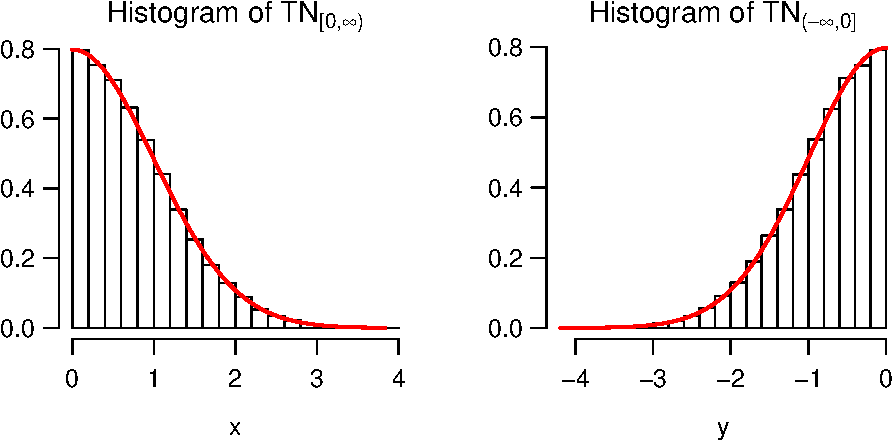
\includegraphics{Hw1_Solution_files/figure-latex/plotTN-1} \end{center}

\section{Question \#3.2}\label{question-3.2}

\subsection{Answer}\label{answer-1}

If \(f(x) = x / 2\), \[
\begin{aligned}
F(x) &= \int_{0}^{x}\dfrac{u}{2}\,\mathrm{d}u = \dfrac{x^{2}}{4},\quad 0\leq x \leq 2\\
F^{-1}(u) &= \sqrt{4u},\quad 0\leq u \leq 1
\end{aligned}
\] Therefore, by the \emph{probability integral transform}, \[
X = F^{-1}(U) = \sqrt{4U},\quad U\sim \operatorname{Unif}(0,1)
\] Analytically, the expected value of \(X\) is \[
\operatorname{E}(X) = \int_{0}^{2}\dfrac{x^{2}}{2}\,\mathrm{d}x = \left.\dfrac{x^{3}}{6}\right|_{0}^{2} = \dfrac{4}{3}
\] Sampling \(X_{1},\ldots,X_{n} \overset{\text{iid}}{\sim} F\), we can
use the law of large numbers to approximate \(\operatorname{E}(X)\),
i.e., \[
\dfrac{1}{n}\sum_{i=1}^{n}X_{i}\xrightarrow{n\to\infty}\operatorname{E}(X)
\]

\begin{Shaded}
\begin{Highlighting}[]
\NormalTok{n =}\StringTok{ }\NormalTok{30000L}
\NormalTok{u =}\StringTok{ }\KeywordTok{runif}\NormalTok{(n, }\DataTypeTok{min =} \DecValTok{0}\NormalTok{, }\DataTypeTok{max =} \DecValTok{1}\NormalTok{)}
\NormalTok{x =}\StringTok{ }\KeywordTok{sqrt}\NormalTok{(}\DecValTok{4} \NormalTok{*}\StringTok{ }\NormalTok{u)}
\NormalTok{Ex =}\StringTok{ }\KeywordTok{mean}\NormalTok{(x)}
\KeywordTok{cat}\NormalTok{(}\StringTok{"E(X) = "}\NormalTok{, }\DecValTok{4}\NormalTok{/}\DecValTok{3}\NormalTok{, }\StringTok{"}\CharTok{\textbackslash{}n}\StringTok{"}\NormalTok{,}
    \StringTok{"Xbar = "}\NormalTok{, Ex, }\DataTypeTok{sep =} \StringTok{""}\NormalTok{)}
\end{Highlighting}
\end{Shaded}

\begin{verbatim}
## E(X) = 1.333333
## Xbar = 1.336276
\end{verbatim}

\section{Question \#3.3}\label{question-3.3}

\subsection{Answer}\label{answer-2}

We know that \(X \sim \operatorname{Laplace}(0,1)\). The inverse CDF (or
the quantile function) of \(\operatorname{Laplace}(0,1)\) is \[
F^{-1}(u) = -\operatorname{sgn}\left(u-\dfrac{1}{2}\right)\log\left(1-2\left|u-\dfrac{1}{2}\right|\right)
\] Therefore, we can plug in \(U\sim \operatorname{Unif}(0,1)\) to
generate random variables from \(\operatorname{Laplace}(0,1)\).

\begin{Shaded}
\begin{Highlighting}[]
\NormalTok{n =}\StringTok{ }\NormalTok{20000L}
\NormalTok{u =}\StringTok{ }\KeywordTok{runif}\NormalTok{(n, }\DataTypeTok{min =} \DecValTok{0}\NormalTok{, }\DataTypeTok{max =} \DecValTok{1}\NormalTok{)}
\NormalTok{DE =}\StringTok{ }\NormalTok{-}\KeywordTok{sign}\NormalTok{(u -}\StringTok{ }\FloatTok{0.5}\NormalTok{) *}\StringTok{ }\KeywordTok{log}\NormalTok{(}\DecValTok{1} \NormalTok{-}\StringTok{ }\DecValTok{2} \NormalTok{*}\StringTok{ }\KeywordTok{abs}\NormalTok{(u -}\StringTok{ }\FloatTok{0.5}\NormalTok{))}
\KeywordTok{par}\NormalTok{(}\DataTypeTok{mfrow =} \KeywordTok{c}\NormalTok{(}\DecValTok{1}\NormalTok{,}\DecValTok{1}\NormalTok{), }\DataTypeTok{mar=}\KeywordTok{c}\NormalTok{(}\FloatTok{3.5}\NormalTok{,}\FloatTok{3.5}\NormalTok{,}\DecValTok{1}\NormalTok{,}\DecValTok{1}\NormalTok{), }\DataTypeTok{mgp=}\KeywordTok{c}\NormalTok{(}\FloatTok{2.4}\NormalTok{,}\FloatTok{0.8}\NormalTok{,}\DecValTok{0}\NormalTok{), }\DataTypeTok{las=}\DecValTok{1}\NormalTok{)}
\KeywordTok{hist}\NormalTok{(DE, }\DataTypeTok{ylab =} \StringTok{""}\NormalTok{, }\DataTypeTok{probability =} \OtherTok{TRUE}\NormalTok{, }\DataTypeTok{breaks =} \DecValTok{20}\NormalTok{,}
     \DataTypeTok{main =} \StringTok{"Histogram of Laplace(0,1)"}\NormalTok{)}
\KeywordTok{curve}\NormalTok{(}\FloatTok{0.5} \NormalTok{*}\StringTok{ }\KeywordTok{exp}\NormalTok{(-}\KeywordTok{abs}\NormalTok{(x)), }\DataTypeTok{from =} \KeywordTok{min}\NormalTok{(DE), }\DataTypeTok{to =} \KeywordTok{max}\NormalTok{(DE), }\DataTypeTok{add =} \OtherTok{TRUE}\NormalTok{, }\DataTypeTok{col =} \StringTok{"red"}\NormalTok{, }\DataTypeTok{lwd =} \DecValTok{2}\NormalTok{)}
\end{Highlighting}
\end{Shaded}

\begin{center}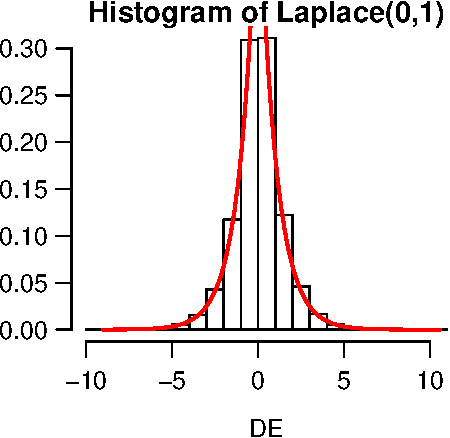
\includegraphics{Hw1_Solution_files/figure-latex/plotExp-1} \end{center}

\section{Question \#3.4}\label{question-3.4}

\subsection{Answer}\label{answer-3}

If \(X \sim f\) is sought but a random variable with density \(g\) is
much easier to generate, we can find \(\beta\) to satisfy a bound on the
densities \[
\beta f(x)\leq g(x)\quad \text{for }0<\beta<1
\] Since we are dealing with a mathematical optimization problem, we can
do without all the constants multiplied, which reduces the objective
function to \[
\hat{x} =\arg\min_{x\in \mathbb{R}} \dfrac{\exp\left(-(x-1/2)^{2}/2\right)}{x^{2}(1-x)^{2}}
\] Moreover, the monotonically increasing function does not affect the
minimizer of the function. Thus, applying the logarithm, \[
\hat{x} = \arg\min_{x\in \mathbb{R}} -\dfrac{1}{2}\left(x-\dfrac{1}{2}\right)^{2} - 2 \log x - 2 \log(1-x)
\] Then by the first-order condition, we find the root of the following
equation \[
-\left(x-\dfrac{1}{2}\right)+\dfrac{2}{1-x}-\dfrac{2}{x} = 0
\] which gives \(x = 1/2\) as the minimizer. Thus, \(\hat{x}=1/2\) and
\(c = 2\). Then, the acceptance-rejection (AR) algorithm goes by

\begin{itemize}
\tightlist
\item
  Generate \(X\) from \(g\).
\item
  Generate \(U\) from \(\operatorname{Unif}(0,1)\).
\item
  If \(Ug(X) \leq \beta f(X)\) then accept \(X\); else reject and repeat
  from the beginning.
\end{itemize}

\begin{Shaded}
\begin{Highlighting}[]
\KeywordTok{library}\NormalTok{(truncnorm)}
\NormalTok{n =}\StringTok{ }\NormalTok{50000L}
\NormalTok{u =}\StringTok{ }\KeywordTok{runif}\NormalTok{(n, }\DataTypeTok{min =} \DecValTok{0}\NormalTok{, }\DataTypeTok{max =} \DecValTok{1}\NormalTok{)}
\NormalTok{tx =}\StringTok{ }\KeywordTok{rtruncnorm}\NormalTok{(n, }\DataTypeTok{a =} \DecValTok{0}\NormalTok{, }\DataTypeTok{b =} \DecValTok{1}\NormalTok{, }\DataTypeTok{mean =} \FloatTok{0.5}\NormalTok{, }\DataTypeTok{sd =} \DecValTok{1}\NormalTok{)}
\NormalTok{u =}\StringTok{ }\KeywordTok{runif}\NormalTok{(n, }\DataTypeTok{min =} \DecValTok{0}\NormalTok{, }\DataTypeTok{max =} \DecValTok{1}\NormalTok{)}
\NormalTok{g =}\StringTok{ }\KeywordTok{dtruncnorm}\NormalTok{(}\DataTypeTok{x =} \NormalTok{tx, }\DataTypeTok{a =} \DecValTok{0}\NormalTok{, }\DataTypeTok{b =} \DecValTok{1}\NormalTok{, }\DataTypeTok{mean =} \FloatTok{0.5}\NormalTok{, }\DataTypeTok{sd =} \DecValTok{1}\NormalTok{)}
\NormalTok{f =}\StringTok{ }\KeywordTok{dbeta}\NormalTok{(tx, }\DecValTok{3}\NormalTok{, }\DecValTok{3}\NormalTok{)}
\NormalTok{M =}\StringTok{ }\KeywordTok{dtruncnorm}\NormalTok{(}\FloatTok{0.5}\NormalTok{, }\DataTypeTok{a =} \DecValTok{0}\NormalTok{, }\DataTypeTok{b =} \DecValTok{1}\NormalTok{, }\DataTypeTok{mean =} \FloatTok{0.5}\NormalTok{, }\DataTypeTok{sd =} \DecValTok{1}\NormalTok{) /}\StringTok{ }\KeywordTok{dbeta}\NormalTok{(}\FloatTok{0.5}\NormalTok{, }\DecValTok{3}\NormalTok{, }\DecValTok{3}\NormalTok{)}
\NormalTok{tx =}\StringTok{ }\NormalTok{tx[u *}\StringTok{ }\NormalTok{g <}\StringTok{ }\NormalTok{M *}\StringTok{ }\NormalTok{f]}
\KeywordTok{par}\NormalTok{(}\DataTypeTok{mfrow =} \KeywordTok{c}\NormalTok{(}\DecValTok{1}\NormalTok{,}\DecValTok{1}\NormalTok{), }\DataTypeTok{mar=}\KeywordTok{c}\NormalTok{(}\FloatTok{3.5}\NormalTok{,}\FloatTok{3.5}\NormalTok{,}\DecValTok{1}\NormalTok{,}\DecValTok{1}\NormalTok{), }\DataTypeTok{mgp=}\KeywordTok{c}\NormalTok{(}\FloatTok{2.4}\NormalTok{,}\FloatTok{0.8}\NormalTok{,}\DecValTok{0}\NormalTok{), }\DataTypeTok{las=}\DecValTok{1}\NormalTok{)}
\KeywordTok{hist}\NormalTok{(tx, }\DataTypeTok{ylab =} \StringTok{""}\NormalTok{, }\DataTypeTok{probability =} \OtherTok{TRUE}\NormalTok{, }\DataTypeTok{breaks =} \DecValTok{20}\NormalTok{,}
     \DataTypeTok{main =} \KeywordTok{TeX}\NormalTok{(}\StringTok{"Histogram of TN$_\{(0,1}\CharTok{\textbackslash{}\textbackslash{}}\StringTok{]\}(0.5, 1)$"}\NormalTok{))}
\KeywordTok{curve}\NormalTok{(}\KeywordTok{dbeta}\NormalTok{(x, }\DecValTok{3}\NormalTok{, }\DecValTok{3}\NormalTok{)}
      \NormalTok{, }\DataTypeTok{from =} \DecValTok{0}\NormalTok{, }\DataTypeTok{to =} \DecValTok{1}\NormalTok{, }\DataTypeTok{add =} \OtherTok{TRUE}\NormalTok{, }\DataTypeTok{col =} \StringTok{"red"}\NormalTok{, }\DataTypeTok{lwd =} \DecValTok{2}\NormalTok{)}
\end{Highlighting}
\end{Shaded}

\begin{center}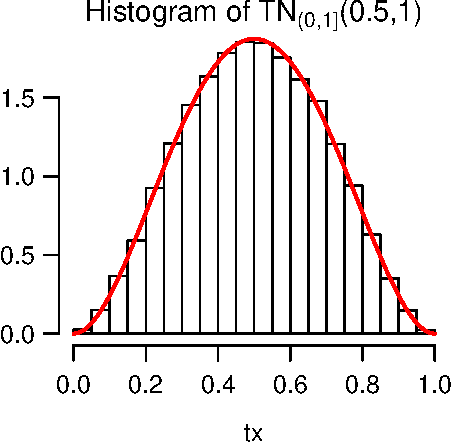
\includegraphics{Hw1_Solution_files/figure-latex/plotTN01-1} \end{center}

\begin{Shaded}
\begin{Highlighting}[]
\KeywordTok{cat}\NormalTok{(}\StringTok{"Var(X) = "}\NormalTok{, }\DecValTok{9} \NormalTok{/}\StringTok{ }\NormalTok{(}\DecValTok{6}\NormalTok{^}\DecValTok{2} \NormalTok{*}\StringTok{ }\DecValTok{7}\NormalTok{), }\StringTok{"}\CharTok{\textbackslash{}n}\StringTok{"}\NormalTok{,}
    \StringTok{"MCvar(X) = "}\NormalTok{, }\KeywordTok{var}\NormalTok{(tx), }\DataTypeTok{sep =} \StringTok{""}\NormalTok{)}
\end{Highlighting}
\end{Shaded}

\begin{verbatim}
## Var(X) = 0.03571429
## MCvar(X) = 0.03586223
\end{verbatim}

\section{Question \#3.6}\label{question-3.6}

\subsection{Answer}\label{answer-4}

To get the minimizer, we need to solve the following optimization
problem: \[
\hat{x} = \arg\min_{x\in \mathbb{R}} \dfrac{x^{2}}{2}-|x|
\] By differentiating the objective function with respect ot \(x\), \[
x - \dfrac{x}{|x|} = 0
\] We get \(x = -1\) or \(x = 1\) as the minimizers. Thus,
\(\hat{x} = -1\) or \(1\) and \(\beta = \sqrt{\pi / (2e)}\) which means
\(c = \sqrt{2e / \pi}\). Thus,

\begin{Shaded}
\begin{Highlighting}[]
\KeywordTok{par}\NormalTok{(}\DataTypeTok{mfrow =} \KeywordTok{c}\NormalTok{(}\DecValTok{1}\NormalTok{,}\DecValTok{1}\NormalTok{), }\DataTypeTok{mar=}\KeywordTok{c}\NormalTok{(}\FloatTok{3.5}\NormalTok{,}\FloatTok{3.5}\NormalTok{,}\DecValTok{1}\NormalTok{,}\DecValTok{1}\NormalTok{), }\DataTypeTok{mgp=}\KeywordTok{c}\NormalTok{(}\FloatTok{2.4}\NormalTok{,}\FloatTok{0.8}\NormalTok{,}\DecValTok{0}\NormalTok{), }\DataTypeTok{las=}\DecValTok{1}\NormalTok{)}
\NormalTok{n =}\StringTok{ }\NormalTok{50000L}
\NormalTok{u =}\StringTok{ }\KeywordTok{runif}\NormalTok{(n, }\DataTypeTok{min =} \DecValTok{0}\NormalTok{, }\DataTypeTok{max =} \DecValTok{1}\NormalTok{)}
\NormalTok{DE =}\StringTok{ }\NormalTok{-}\KeywordTok{sign}\NormalTok{(u -}\StringTok{ }\FloatTok{0.5}\NormalTok{) *}\StringTok{ }\KeywordTok{log}\NormalTok{(}\DecValTok{1} \NormalTok{-}\StringTok{ }\DecValTok{2} \NormalTok{*}\StringTok{ }\KeywordTok{abs}\NormalTok{(u -}\StringTok{ }\FloatTok{0.5}\NormalTok{))}

\NormalTok{u =}\StringTok{ }\KeywordTok{runif}\NormalTok{(n, }\DataTypeTok{min =} \DecValTok{0}\NormalTok{, }\DataTypeTok{max =} \DecValTok{1}\NormalTok{)}
\NormalTok{M =}\StringTok{ }\FloatTok{0.5} \NormalTok{*}\StringTok{ }\KeywordTok{exp}\NormalTok{(-}\DecValTok{1}\NormalTok{) /}\StringTok{ }\KeywordTok{dnorm}\NormalTok{(}\DecValTok{1}\NormalTok{)}
\NormalTok{stdNormal =}\StringTok{ }\NormalTok{DE[u *}\StringTok{ }\NormalTok{(}\FloatTok{0.5} \NormalTok{*}\StringTok{ }\KeywordTok{exp}\NormalTok{(-}\KeywordTok{abs}\NormalTok{(DE))) <=}\StringTok{ }\NormalTok{M *}\StringTok{ }\KeywordTok{dnorm}\NormalTok{(DE)]}
\KeywordTok{hist}\NormalTok{(stdNormal, }\DataTypeTok{probability =} \OtherTok{TRUE}\NormalTok{,}
     \DataTypeTok{main =} \StringTok{"Histogram of Standard Normal"}\NormalTok{, }\DataTypeTok{ylab =} \StringTok{""}\NormalTok{, }\DataTypeTok{xlab =} \StringTok{"x"}\NormalTok{)}
\KeywordTok{curve}\NormalTok{(}\KeywordTok{dnorm}\NormalTok{(x), }\DataTypeTok{from =} \KeywordTok{min}\NormalTok{(stdNormal), }\DataTypeTok{to =} \KeywordTok{max}\NormalTok{(stdNormal),}
      \DataTypeTok{add =} \OtherTok{TRUE}\NormalTok{, }\DataTypeTok{col =} \StringTok{"red"}\NormalTok{, }\DataTypeTok{lwd =} \DecValTok{2}\NormalTok{)}
\end{Highlighting}
\end{Shaded}

\begin{center}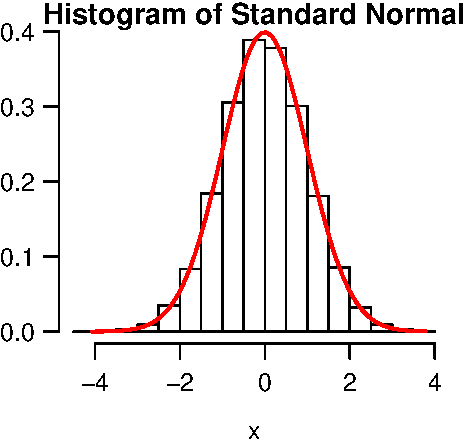
\includegraphics{Hw1_Solution_files/figure-latex/plotSNcompare-1} \end{center}

\begin{Shaded}
\begin{Highlighting}[]
\KeywordTok{cat}\NormalTok{(}\StringTok{"E(x) = "}\NormalTok{, }\KeywordTok{mean}\NormalTok{(stdNormal), }\StringTok{"}\CharTok{\textbackslash{}n}\StringTok{"}\NormalTok{,}
    \StringTok{"Var(x) = "}\NormalTok{, }\KeywordTok{var}\NormalTok{(stdNormal), }\DataTypeTok{sep =} \StringTok{""}\NormalTok{)}
\end{Highlighting}
\end{Shaded}

\begin{verbatim}
## E(x) = -0.007003033
## Var(x) = 0.9921894
\end{verbatim}

\newpage
\singlespacing 
\end{document}
